\documentclass[11pt]{article}\usepackage[sc]{mathpazo} %Like Palatino with extensive math support
\usepackage{fullpage}
\usepackage[authoryear,sectionbib,sort]{natbib}\linespread{1.7}
\usepackage[utf8]{inputenc}
\usepackage{lineno}\usepackage{titlesec}
\titleformat{\section}[block]{\Large\bfseries\filcenter}{\thesection}{1em}{}
\titleformat{\subsection}[block]{\Large\itshape\filcenter}{\thesubsection}{1em}{}
\titleformat{\subsubsection}[block]{\large\itshape}{\thesubsubsection}{1em}{}
\titleformat{\paragraph}[runin]{\itshape}{\theparagraph}{1em}{}[. ]\renewcommand{\refname}{Literature Cited}
\usepackage{biblatex}
\addbibresource{References.bib}
\newcommand{\tom}[2]{{\color{red}{#1}}\footnote{\textit{\color{red}{#2}}}}
\newcommand{\ali}[2]{{\color{pink}{#1}}\footnote{\textit{\color{pink}{#2}}}}  
%% Following is used only for line numbers for pre-acceptance submissions
\usepackage{lineno}
%%%%%%%%%%%%%%%%%%%%%
% Line numbering
%%%%%%%%%%%%%%%%%%%%%
%
% Please use line numbering with your initial submission and
% subsequent revisions. After acceptance, please turn line numbering
% off by adding percent signs to the lines %\usepackage{lineno} and
% to %\linenumbers{} and %\modulolinenumbers[3] below.
%
% To avoid line numbering being thrown off around math environments,
% the math environments have to be wrapped using
% \begin{linenomath*} and \end{linenomath*}
%
% (Thanks to Vlastimil Krivan for pointing this out to us!)

\title{An Integral Projection Modeling Approach to Demographic Consequences of Multiple Partner Mutualisms }

% This version of the LaTeX template was last updated on
% May 11, 2023.

%%%%%%%%%%%%%%%%%%%%%
% Authorship
%%%%%%%%%%%%%%%%%%%%%
% Please remove authorship information while your paper is under review,
% unless you wish to waive your anonymity under double-blind review. You
% will need to add this information back in to your final files after
% acceptance.

\author{Alexandra Campbell$^{1,\ast}$ \\ 
Tom E.X. Miller$^{1,\dag}$}

\date{}

\begin{document}

\maketitle

\noindent{} 1. Rice University, Houston, Texas 77004;

\noindent{} $\ast$ Corresponding author; e-mail: amc49@rice.edu.

\noindent{} $\dag$ Corresponding author; e-mail: tom.miller@rice.edu.

\textit{Manuscript elements}: Figure~1, figure~2, table~1, appendix~A (for print; including figure~A1, figure~A2, and table~A1), supplemental PDF. Figure~2 is to print in color.

\bigskip

\textit{Keywords}: Examples, model, template, guidelines.

\bigskip

\textit{Manuscript type}: Article.

\bigskip

\noindent{\footnotesize Prepared using the suggested \LaTeX{} template for \textit{Am.\ Nat.}}

%% Comment out the following two lines after acceptance
\linenumbers{}
\modulolinenumbers[3]

\newpage{}
\section*{Abstract}  
  Mutualisms are among the most widespread species interactions with diverse and dynamic consequences. They are considered more context dependent than other species interactions, meaning there are many different factors which influence the impacts of a mutualistic interaction, including partner diversity. Partner diversity has become a central focus in the field of mutualisms in recent years shifting the focus to multispecies mutualisms where the focus was previously on pairwise studies. It has been shown that pairwise studies are poor predictors of the effects of multispecies mutualistic interactions. The diversity of partners in a multi-species mutualism causes varied demographic effects on the population of the focal mutualist which can be explained by several mechanisms, portfolio effect, complementarity, and sampling effect. In this paper, I will focus on defensive ant-plant mutualisms. These involve plants which provide extra-floral nectar and/or “housing” to ants which in turn defend them from herbivores. While these interactions have been well studied in the literature, few have considered how diversity within partner guilds affect the overall benefits of mutualism for the plant partner.   
  I use the plant, Cylindropuntia imbracata (tree cholla), and ant, Crematogaster opuntiae (Crem.), Liometopum apiculatum (Liom.), and more, multispecies mutualism in which the cacti provide extrafloral nectar in exchange for defense from various herbivores and seed predators. I used 18 years of data collected from demographic censuses, which includes data such as size, survival, reproductive status, flowers produced, ant partner, and herbivory for 8 30x30 m plots, in New Mexico. With this data I parameterize a series of Bayesian generalized linear vital rate models to determine the impacts of different partners on the focal mutualists. I found that different ant partners did have different impacts on the vital rates of the tree cholla. Specifically, Crem. tended plants had advantages in both growth and survival when small, and Liom. tended plants had advantages in colonizing partners as well as floral viability. With these models I constructed an Integral Projection Model in which I could vary the presence of each partner, creating different “diversity scenarios”, to determine under which diversity scenario the focal mutualist experienced the highest fitness, and which of the above mechanisms may explain the effects of partner diversity in this system. I found that the real-life scenario (all possible ants are present) lead to the highest fitness for the tree cholla, indicating that partner diversity is beneficial in this system. It also shows that complementarity is at play in this system, meaning different partners offer different benefits leading to synergistic benefits for the tree cholla. 

\newpage{}
\section*{Introduction}
  Mutualisms are species interactions where all participants benefit, leading to higher individual fitness and increased population growth rates. They are among the most widespread species interactions\cite{Chamberlain2014, BoucherDouglasH.1985} with diverse and dynamic consequences \cite{Bronstein1994,Chamberlain2014,Frederickson2013}, often deteriorating into other types of interactions, including parasitism \cite{Rodriguez-Rodriguez2017,Song2020,Mandyam2014,Thrall2007, Bahia2022}.One reason they are so ubiquitous is they take many forms in nature, including defense for food or housing\cite{Willmer1997}, pollination and dispersal for food\cite{Sakai2002,Burns2004}, resource uptake for housing\cite{Holland2010}, etc. Mutualisms are typically considered more context dependent than other species interactions\cite{Chamberlain2014,Frederickson2013}, meaning strength of the interaction is often determined by the surrounding environment and species. Historically, pairwise studies, where two species engage in mutualism with only each other, were central in the field of mutualisms, it has since been shown that pairwise studies are poor predictors of the effects of multi-species mutualistic interactions\cite{Afkhami2014,Palmer2010}, where more than two species engage in mutualisms.The differences in mutualistic outcomes are due to differences in partner quality\cite{Bascompte2019,Stanton2013,Frederickson2013,Jones2015, Ness2006}, differences in the types of benefits offered\cite{Kiers2003,Afkhami2014}, and direct interactions between partners\cite{Sun2019,Heath2009,Heath2014,Grutter2003}.For these reasons, pairwise studies cannot be accurately used to predict the outcomes of multi-species mutualisms\cite{Palmer2010, Stanton2013, Chamberlain2014, Song2020}.Studies on the effects of diverse multi-species mutualism systems are necessary to help us understand the demographic effects of partner diversity in mutualisms\cite{Bascompte2019}. Multi-species mutualism partner diversity causes varied demographic effects on the population of the focal mutualist which can be explained by a number of mechanisms.\ali{In some cases, the quality of the benefits offered varies leading to some partners which benefit the individual, some which have neither a positive or negative impact on the individual, and some which negatively impact the host}{Is this the best way to introduce this or should I talk about quality of benefits compared to cost of rewards? AKA some partners offer a net benefit when the benefits outweigh the cost of rewards to the partner ... etc.} \cite{Bronstein1994,Bronstein2001a,Afkhami2014,Song2020,West2007,Frederickson2013,Jones2015}. In cases where the partner offers benefits, \ali{the function, or type of benefits, offered by the partner can vary}{Is this enough detail or do I need to go into examples?} \cite{Stanton2003}.
  
  \begin{figure}[h]
    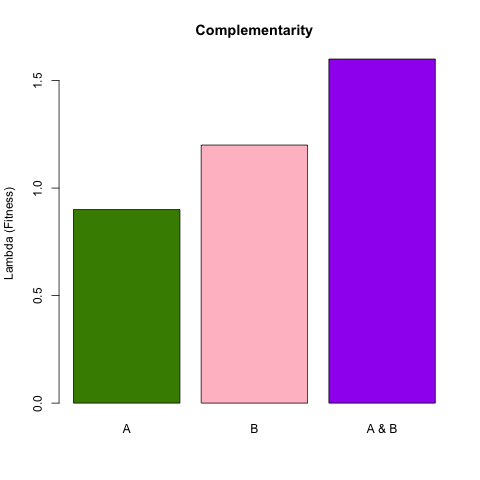
\includegraphics[width=0.58\linewidth]{Complementarity copy.png}
    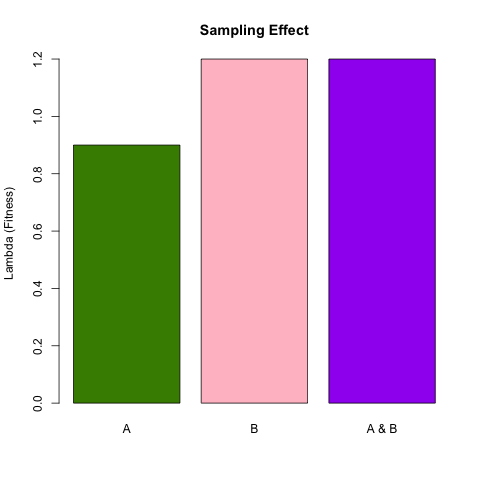
\includegraphics[width=0.40\linewidth]{Sampling_Effect copy.png}\caption{asdasdf}\label{fig:comp-samp}
  \end{figure}
  \begin{figure}[h]
    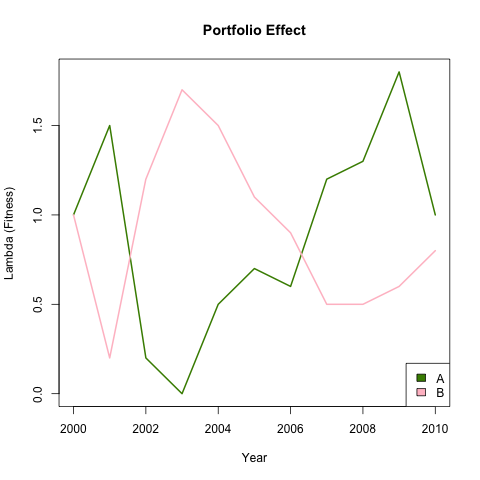
\includegraphics[width=0.60\linewidth]{Portfolio_Effect copy.png}
    \caption{asdasdf}
    \label{fig:portfolio}
  \end{figure}
  
  This variation in partners can lead to \ali{net benefits, no net benefits, or net costs for the focal mutualist}{Is this the best way to start this paragraph? If so should I include a figure panel?}.In this study I focus on the positive effects of partner diversity which can be explained by several mechanisms described below. When there is a consistent partner hierarchy based on benefits offered, a more diverse sample of the partner community may be more likely to include the highest quality partner (the one which offers the focal mutualist the most benefit)\cite{Frederickson2013}.When this leads to the fitness of a focal mutualist interacting with multiple partners being equal to the fitness of a focal mutualist interacting with only the highest quality partner, as shown in Figure \ref{fig:comp-samp}b, sampling effect can explain the positive effects of partner diversity\cite{Batstone2018}. Partners can also vary functionally, meaning each partner offers a different type of reward to the focal mutualist\cite{Stachowicz2005,Bronstein2006,Stanton2003}.When this leads to a higher fitness for the focal mutualist than any single interaction,as shown in Figure \ref{fig:comp-samp}a, complementarity explains the benefits of partner diversity\cite{Batstone2018}. Partners can also have asynchronous responses to the environment, either spatially\cite{Ollerton2006} or temporally\cite{Alarcon2008}.Multiple partners can act as a 'portfolio' leading to more even fitness benefits across environmental or temporal heterogeneity, as shown in Figure \ref{fig:portfolio}, through the portfolio effect\cite{Batstone2018,Lazaro2022}.Partner diversity can have different effects depending on whether partners are present all at once or sequentially (partner turnover) \cite{Djieto-Lordon2005, Ness2006, Bruna2014}. Turnover can happen at different timescales\cite{Oliveira1999,Horvitz1986} from minutes to years. The degree and order of partner turnover can have important impacts on the fitness of the focal mutualist.\ali{The degree, or rapidity, of partner turnover can impact the level of benefits recieved by the focal mutualist particularly if the benefits continue to accumulate or if they saturate over time \cite{Sachs2004}.}{Not quite sure what to say here. } The direction of turnover can also have a significant impact, particularly if the most beneficial partner changes across the ontogeny of the focal mutualists life\cite{Fonseca2003}.For example, susceptibility to enemies can change across life stages\cite{Boege2005,Barton2010} so the focal mutualist benefits the most when defensive partners align with the more vulnerable life stages of focal mutualists \cite{Djieto-Lordon2005}.\ali{Ant visitation to extra-floral nectar producing plants are a classic and well-studied example of interspecific mutualisms which are often multispecies and have dynamic turnover patterns}{... Is this a better transition? I tried to tie it in a bit more conceptually.}, making these interactions great systems to study the effects of partner diversity.A subset of these interactions, defensive ant-plant mutualisms are common interactions in which plants provide food and/or ``housing'' to ants which in turn defend them from herbivores\cite{Bronstein1998, Bronstein2006}. While these interactions have been well studied\cite{Ness2006,Beattie1985,Schultheiss2022}, few have considered how diversity within ant defender guilds\cite{Stanton2013} or temporal fluctuations in partner interactions\cite{Trøjelsgaard2015} affect the overall benefits of mutualism for the plant partner.This study focuses on the tree cholla cactus, a long lived \textit{Cylindriopuntia imbricata}, EFN-bearing plant that associates with multiple species of ant partners.Insect herbivory negatively affects the growth of cholla, in turn reducing population growth rates\cite{Miller2009}. Ant partners defend the cholla from these insect herbivores, reducing the negative effects of herbivory\cite{Miller2007}. The multiple ant partners do not co-occur on individual plants, but a single cholla may interact with multiple types of partners over its lifetime.While the quality of ant partners in this system has been studied, with some seen as superior defenders and some  being viewed as net-negative because they can deter pollinators \cite{Ohm2014}, no one has integrated demographic effects over the life cycle of these tree cholla.
  
  \begin{figure}[h]	
    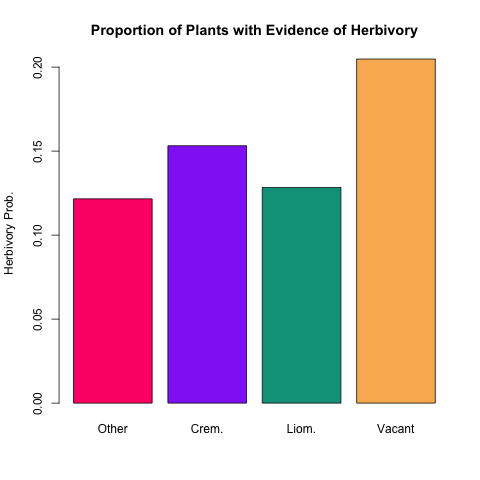
\includegraphics[width=.8\linewidth]{herb_ant_only_flow.png}	
    \caption{asdasdf}	
    \label{fig:herb}
  \end{figure}
  
  In this study we will answer three questions about the demographic effects of partner diversity across host lifetimes in multi-species mutualisms:
  \begin{enumerate}	
    \item{What are the contrasting demographic effects of multiple partners?}	
    \item{How do host size and partner identity impact the directionality of turnover between multiple           partners?}	
    \item{What mechanisms explain the effects of partner diversity in a multispecies mutualism?}
    \end{enumerate}
    To answer these questions, we used a 20-year long-term dataset of individual-level demographic information and ant partner identity and quantity data to track the structure of the population across time as well as individual level impacts of ant partners on the cacti.We used vital rate functions to evaluate the first two questions. We then used the composite integral projection model (IPM) to evaluate how vital rate differences affect intrinsic population growth rates and identify mechanisms at play. 
    
  \section*{Methods}
  \subsection*{Study System}
  This study was conducted in the Los Pi$\tilde{n}$os mountains, a small mountain chain located on the Sevilleta National Wildlife Refuge, a Long-term Ecological Research (LTER) site in central New Mexico.
This is an area characterized by steep, rocky slopes, and perennial vegetation like cacti and junipers. 
Tree cholla cacti are common in high Chihuahuan desert habitats, with their native range spanning the southwestern USA\cite{Benson1982}. 
These arborescent cholla produce cylindrical segments with large spines. 
In the growing season, May to August in New Mexico, the plants initiate new vegetative segments and flower buds at the ends of existing segments. 
While most plants produce new segments every season, only those which are reproductively mature produce flower buds. 
Tree cholla generally reach at least 9 years of age before beginning to reproduce \cite{Ohm2014}.
Like other EFN-bearing cacti, tree cholla secrete nectar from specialized glands on young vegetative and reproductive structures\cite{Ness2006,Oliveira1999}.

  This EFN is harvested by various ant species in return for defense. 
At the Sevilleta, the cholla are visited primarily by two species of ground-nesting ants from the formicoid clade, \textit{Crematogaster opuntiae} and \textit{Liometopum apiculatum}, as well as other rarer species, including \textit{Forelius pruinosus}, a \tom{\textit{Phenogaster spp.}}{Incorrect spelling.}, and \textit{Camponotus spp.}.
\textit{L. apiculatum} are the most frequent visitors with $25\% - 60\%$ of tree cholla tended by these ants, followed by \textit{C. opuntiae} visiting between $0\% - 20\%$ of cacti\cite{Donald2022} depending on the year. Up to $80\%$ of cacti remain vacant in any given year. 

  These ants rarely co-occur on a plant, probably due to interspecific competition\cite{Miller2007}.
Each cholla is visited by a single ant species for the duration of a season, and the species of the visitors can change from one season to the next. 
At the beginning of the growing season, when EFN production begins, the ground-nesting ants will begin visiting tree cholla.
They will visit the cholla every day during the season around the clock, with the most acticity around sunrise or sunset\cite{Ohm2014}. 
Smaller cholla are less likely to be visited because they produce very little EFN, so larger cholla are generally more highly tended\cite{Miller2014}. 
In late August, the tree cholla stop producing EFN and the ants vacate until the next growing season. 

  There are a variety of insect herbivores and seed predators which attack the cholla, focusing either on the vegetative segments and the reproductive segments\cite{Mann1969}. 
An unidentified weevil of the genus \textit{Gerstaekeria} feeds on vegetative and reproductive structures and implants their larvae within the plant tissue for the winter. 
A cactus bug, \textit{Narnia pallidicornis}, (Hemiptera: Coreidae) feeds on all cholla parts with a preference for the reproductive structures \cite{Miller2006}.
A seed predator, \textit{Cahela ponderosella}, (Lepidoptera: Pyralidae) attacks developing fruits pre-dispersal and oviposits in open flowers mid-growing season where larvae burrow into the ripening ovary. 
These predators can have significant negative impacts on the fitness of individual cholla and depress population growth\cite{Miller2009}.
There is experimental evidence that tree cholla tended by \textit{L. apiculatum} and \textit{C. opuntiae} experience less herbivory from all of the mentioned insect predators\cite{Miller2007}. 

	\subsection*{Data}
The data collected are from a long-term dataset spanning 2004 to 2023 taken from 30 $\times$ 30 meter plots at the Sevilleta LTER. 
The data initially included 134 naturally occurring plants across 4 spatial blocks censused annually from 2004 to 2008.
Six of the plots were established in 2009 by tagging all existing plants within a 30 $\times$ 30 meter area. 
The final two plots were added to this census from 2011 onwards. 
Annually, in May we surveyed these plots, taking many types of demographic and partner data. 
For each cholla, we recorded plant survival from the last survey to the current survey. 
We recorded the height (cm), maximum crown width, and crown width perpendicular to the maximum, which are used to calculate plant volume ($cm^3$) based on the volume of a cone with the mean of maximum crown width and perpendicular crown width as the diameter. 
We recorded the total number of flower buds, including how many were aborted and how many were not. We recorded all ant species present and the number of ants we could count in 30 seconds. 
We also recorded the species of herbivore and the number present on the plant.
		
	\subsection*{Statistical Modeling -- Construction}
  With the data described above we fit a series of generalized linear mixed models (GLMMs) in a hierarchical Bayesian framework with both fixed and random effects.
Many of the vital rates are estimated as a function of plant size, ant partner, or both.
Ant partner type is included as a predictor only where there are biological pathways through which ants could impact the outcome of that process. 
The biological sources of variance (including individual, spatial, and annual variance) are accounted for by including year-to-year and plot-to-plot random effects in the models. 
Unless otherwise mentioned, all models use vague priors. 
The growth model ($G_j(y,x)$) estimates the size of cholla, with fixed effects of the previous size and ant partner and random effects of plot and year, using a Skew Normal distribution, with $\omega$ and $\alpha$ varying with the previous size. 
Ants are included as a predictor here because ant partners defend plants from herbivory, therefore decreasing the likelihood of segment loss.
The survival model ($S_j(x)$) estimates the probability of survival, with fixed effects of the previous size of the cholla and ant partner and random effects of plot and year, using a Bernoulli distribution. 
Ants are included as predictors here because ant partners defend cholla from herbivores and predators, decreasing the likelihood of mortality due to either of these. 
The reproduction model ($P(x)$) estimates the probability of reproducing each year, with fixed effects for the size and random effects of plot and year, using a Bernoulli distribution. 
The total flowers model ($F(x)$) estimates the total flowers produced by a plant, with fixed effects of size and random effects of plot and year, using a Negative Binomial distribution. 
The viability model ($V_i(x)$) estimates the proportion of flowers produced by a plant which are viable (not aborted), with fixed effects of the ant partner of the cactus and random effects of plot and year, using a Binomial distribution.
Ants are included as predictors here because they defend the cacti from seed predation which can lead to floral abortion. 
The ant transition rates model ($\tau_{i,j}(x)$) estimates the probability of a cactus being visited by an ant partner, with fixed effects of the previous size of the cholla and the previous ant partner and random effects of plot and year, using a Multinomial distribution.  
Ant partners are included as predictors here because partners may choose to return to the same cholla repeatedly or choose new ones, therefore the previous partner may be a good indicator of the next partner. 
The recruit size model ($n_j(x)$) estimates the size distribution of all recruits from a given year, with no fixed or random effects, using a Normal distribution. 
With germination data from Miller et al., 2009, we fit two Bayesian generalized linear models for the probability of germinating from a seed in the first year ($\gamma_1$) or the second year ($1 - \gamma_1$), with no fixed or random effects, using a Binomial distribution.
With data collected in a 2005-2006 recruit census, we fit a Bayesian generalized linear model for the probability of a seedling surviving to May ($\delta$) (accounting for missed mortality events), with fixed effects of the previous size and random effects of the transect, using a Bernoulli distribution. 
With data from Miller 2007, we fit a Bayesian generalized linear model for the number of seeds produced by every flower on a cholla ($\kappa$) based on the ant partner, using a Negative Binomial distribution. 
Ant partners are included as predictors here because they reduce floral abortion rates and therefore may lead to higher numbers of seeds. 

  To obtain posterior estimates of the demographic parameters, we fit models using Markov chain Monte Carlo (MCMC) simulations via STAN run through version 4.0.2 of R 
For each model, we obtained 3 chains of 10,000 iterations, each with randomly chosen initial conditions. 
The first 1,500 iterations were discarded as burn-in to eliminate transience associated with initial conditions. 
We did not thin the chains, thus all samples were retained. 
To assess the convergence of our models we assessed between and within chain convergence, the resulting figures are included in supplemental documents. 
To assess the overall model fit we carried out posterior predictive checks to examine how well the fitted model can generate simulated data similar to the real data.
Large differences in the two indicate a poor model fit and can be assessed visually (figures included in supplemental documents). 
All estimated parameters are described in table 1.
Data and code for all vital rate models is included in the supplemental information.

  \subsection*{Integral Projection Model Construction}
  Integral Projection Models describe population dynamics in discrete time, with continuous functions that relate vital rates to continuous and discrete state variables. 
We constructed a composite IPM which allows us to analyze the long term population growth rate of cholla with ant transition dynamics explicitly included.
Many of the vital rate models are dependent not only on continuous size variables, but also on discrete variables representing the ant partner present.
There is also a transition rate which determines what proportion of cholla are tended by each ant in a given year based on the previous ant partner and the size of the plants. 
This unique composite structure allows us to determine the individual effects of each ant species as well as the composite effects of several partners across the cholla population. 

  Following previous studies, we modeled the life cycle of cholla using continuously size-structured plants, $n_i(x)$, where x is the size of the cholla and i is the ant partner, and two discrete seed banks ($B_{1,t}$ and $B_{2,t}$) corresponding to 1 and 2-year old seeds.
The dynamics of these 1 and 2-year old seedbanks are given by the following equations: 

  \begin{linenomath*}
		$$
		B_{1, t+1} = \kappa \delta \sum_{i}^{4} \int_L^U P(x) V_i(x) F(x) n_i(x) dx \\
		$$
		$$
		B_{2,t+1} =  (1 - \gamma_1)B_{1,t}\\
		$$
  \end{linenomath*}

  The functions $P(x)$ and $F(x)$ give the probability of flowering, the number of flowerbuds produced based on the plant size $x$ and the year $t$. 
The proportion of flowerbuds which will produce seeds ($V_i(x)$) is dependent on the plant size $x$ and the ant species present on the plant $i$ in year $t$. 
The integral is multiplied by the number of seeds per fruit ($\kappa$) and the probability of seed dispersal/survival ($\delta$) to give the number of seeds that enter the one-year old seed bank. 
Parameters $U$ and $L$ are the upper and lower bounds, respectively, of the plant size distribution. 
Plants can recruit out of the one-year seed bank with the probability of $\gamma_1$ or transition to the two-year seed bank with a probability of $1 - \gamma_1$. 
Seeds in the two-year seed bank are assumed to either germinate with a probability of $\gamma_2$ or die. 
		
  The size dynamics of the cholla are given by:
		
	\begin{linenomath*}
		$$
		n(y,i)_{t+1} = (\gamma_1 B_{1,t} + \gamma_2 B_{2,t}) \eta(y) \omega \beta_i  + \\
		$$
		$$
		\sum_{j}^{4} \int_L^U S_j(x) G_j(y,x) \tau_{ij}(x) n_j(x) dx \\
		$$
	\end{linenomath*}
	
  The first term gives the recruitment from one and two-year seed banks to a plant of size $y$, where $\eta(y) ~ N(***)$ gives the seedling size distribution and $\omega ~ ***$ gives the proportion of seedlings which surive from germination (late summer) to the census (May).
The second term reflects the changes in the population of the cholla which are not recruits, where $S_j(x)$ gives the probability of a plant of size $x$ in year $t$ surviving to year $t+1$ with partner $j$.
$G_j(y,x)$ gives the probability of growing from size $x$ in year $t$ to size $y$ in year $t+1$, respectively with partner $j$. 
Finally, $\tau_{ij}$ is the probability of a cholla which is size $x$ with ant partner $i$ in year $t$ being tended by ant partner $j$ in year $t+1$.

  \subsection*{Deterministic IPM Analysis}
  Analyzing an IPM requires discretizing the composite IPM into a matrix to calculate the dominant eigenvalue. 
Each component of the IPM (each set of ant partner specific vital rates) can be discretized into its own $ 200 \times 200$ matrix \as shown in figure ***. 
The possibility of eviction, when individuals are predicted to grow outside of the possible size classes, was avoided by adding probabilities of growing smaller or larger than the existing boundaries, as done by many others***.
We used the composite IPM to quantify the effects of partner diversity on the intrinsic growth rate of cholla, $r$ $ln(\lambda)$. 
We calculated the $r$ for each combination of ant partners: complete vacancy; \textit{L. apiculatum} and vacancy; \textit{C. opuntiae} and vacancy; other and vacancy; \textit{L. apiculatum}, \textit{C. opuntiae}, and vacancy, \textit{L. apiculatum}, other, and vacancy; \textit{C. opuntiae}, other, and vacancy; and all ant partners and vacancy.
The relative distributions allowed us to determine if either complementarity or sampling effect were at play in the tree cholla-ant defense system.
Sampling Effect requires that the $r$ when all possible partners are present is equal to the $r$ of the cholla population when only the best partner is present.
Complementarity requires that the $r$ when all possible partners are present is greater than the $r$ of any other combination of partners or any single partner. 


  \subsection*{Stochastic IPM Analysis}
  The third mechanism considered in this study requires annual variation to be explicitly considered in the IPM so we constructed a stochastic version of the IPM described above. 
The year of record was a random effect in all vital rate models meaning we were able to include an intercept for specific years. 
In order to include stochasticity in the analysis, we randomly sampled from the year-random effect intercepts 1,000 times.
For each of these 1,000 iterations we calculated the $r$ for every possible combination of ant partners. 
With these values we calculated $\delta r$ between the scenario with all possible partners and the scenario with no partners.
This $\delta r$ measures the net benefits offered by partner diversity with annual variation.
We also calculated the $\delta r$ of the deterministic IPM to measure the net benefits offered by partner diversity without annual variation. 
These two relative differences allow us to determine if portfolio effect is at play.
Portfolio effect is demonstrated when the net benefit with annual variation is larger than the net benefit without annual variation. 
		
% I am creating a table here to include all parameter estimations and descriptions
  \begin{table}[]
  \begin{tabular}{l|l|l}
    \textbf{Parameter} & \textbf{Median ($95\%$ CI)} & \textbf{Prior Distribution} \\
    \hline
    %% Growth Parameters
    growth xi intercept vacant $\Beta_01^g$ & -5.210899 (-5.686865, -5.491787) & \\
    growth xi intercept other $\Beta_02^g$ & -5.8288 (-5.956217, 1.766021) & \\
    growth xi intercept \textit{C. opuntiae} $\Beta_03^g$ & -4.529523 (-6.0770390, 0.1222112) & \\
    growth xi intercept \textit{L. apiculatum} $\Beta_04^g$ -5.106802 (-5.4499944, 0.5453901) & \\
    growth xi size dependent vacant $\Beta_11^g$ & & \\
    growth xi size dependent other $\Beta_12^g$ & & \\
    growth xi size dependent \textit{C. opuntiae} $\Beta_13^g$ & & \\
    growth xi size dependent \textit{L. apiculatum} $\Beta_14^g$ & & \\
    growth omega intercept $\omega_0^g$ & & \\
    growth omega size dependent $\omega_1^g$ & & \\
    growth alpha intercept $\alpha_0^g$ & & \\
    growth alpha size dependent $\alpha_1^g$ & & \\
    \hline
    %% Germination Parameters
    1-year germination intercept $\alpha^{\gamma_1}$ & & \\
    2-year germination intercept $\alpha^{\gamma_2}$ & & \\
    \hline
    %% Survival Parameters
    survival intercept vacant $\Beta_01^s$ & & \\
    survival intercept other $\Beta_02^s$ & & \\
    survival intercept \textit{C.opuntiae} $\Beta_03^s$ & & \\
    survival intercept \textit{L. apiculatum} $\Beta_04^s$ & & \\
    survival size dependent vacant $\Beta_11^s$ & & \\
    survival size dependent other $\Beta_12^s$ & & \\
    survival size dependent \textit{C. opuntiae} $\Beta_13^s$ & & \\
    survival size dependent \textit{L. apiculatum} $\Beta_14^s$ & & \\
    \hline
    %% Probability of Flowering Parameters
    flowering intercept $\Beta_0^f$ & & \\
    flowering size dependent $\Beta_1^f$ & & \\
    \hline
    %% Floral Viability Parameters
    viability intercept vacant $\Beta_01^v$ & & \\
    viability intercept other $\Beta02^v$ & & \\
    viability intercept \textit{C. opuntiae} $\Beta_03^v$ & & \\
    viability intercept \textit{L. apiculatum} $\Beta_04^v$ & & 
  \end{tabular}
  \end{table}
			
    
  
    
%%%%%%%%%%%%%%%%%%%%%
% Acknowledgments
%%%%%%%%%%%%%%%%%%%%%
% You may wish to remove the Acknowledgments section while your paper 
% is under review (unless you wish to waive your anonymity under
% double-blind review) if the Acknowledgments reveal your identity.
% If you remove this section, you will need to add it back in to your
% final files after acceptance.

\section*{Acknowledgments}

OEC would like to thank Madlen Wilmes, Gyuri Barab\'{a}s, Flo D\'{e}barre, Vlastimil K\v{r}ivan, and Greg Dwyer for their comments and suggestions on this template.

%%%%%%%%%%%%%%%%%%%%%
% Statement of Authorship
%%%%%%%%%%%%%%%%%%%%%
% This section should also be commented out while your MS is undergoing
% double-blind review. The specifics should of course be adapted to
% your paper, but the paragraph below gives some hints of possible
% contributions.

\section*{Statement of Authorship}

OEC conceived the experiments, collected the data, and wrote the original draft.
GHC provided specimens and analyzed the model.
AQE oversaw data analysis and developed the code. 
All authors reviewed and edited the writing at all stages of revision.

\section*{Data and Code Availability}

On initial submission, you may use this section to provide a URL for editors and reviewers that is `private for peer review'. After acceptance, this section must be updated with correct, working DOIs for data deposits (such as on the Dryad Digital Repository, \citealt{CookEtAl2015}) and code deposits (such as in Zenodo). 

\section*{Appendix A: Additional Methods and Parameters}

% In most cases, authors should typeset supplementary material in a separate,
% author-supplied PDF. For author-supplied PDFs, please consult the
% AmNat_supp_template.tex document, available from
% https://www.journals.uchicago.edu/journals/an/instruct 
%
% By contrast, the Appendix instructions below apply to cases in which
% a brief appendix is to appear in print after the main body of the article.
% That notably includes descriptions of methods, tables defining parameters,
% and other material necessary for reproducing the MS's results.
%
% Please reset counters for the appendix (thus normally figure A1, 
% figure A2, table A1, etc.).
%
% Most AmNat articles have no more than one print appendix. If your article
% has more than one, counters for each appendix should match the letter of
% that appendix. For example, tables in Appendix B should be numbered table B1, % table C2, etc. This applies to tables, equations, and figures.
%
% It's better not to use the \appendix command, because we have some
% formatting peculiarities that \appendix conflicts with.

\renewcommand{\theequation}{A\arabic{equation}}
% redefine the command that creates the equation number.
\renewcommand{\thetable}{A\arabic{table}}
\setcounter{equation}{0}  % reset counter 
\setcounter{figure}{0}
\setcounter{table}{0}

\subsection*{Fox--dog encounters through the ages}

The quick red fox jumps over the lazy brown dog. The quick red fox has always jumped over the lazy brown dog. The quick red fox began jumping over the lazy brown dog in the 19th century and has never ceased from so jumping, as we shall see in figure~\ref{Fig:Jumps}. But there can be surprises (figure~\ref{Fig:JumpsOk}).

If the order and location of figures is not otherwise clear, feel free to include explanatory dummy text like this:

[Figure A1 goes here.]

[Figure A2 goes here.]

\subsection*{Further insights}

Tables in the appendices can appear in the appendix text (see table~\ref{Table:Rivers} for an example), unlike appendix figure legends which should be grouped at the end of the document together with the other figure legends.

\begin{table}[h]
\caption{Various rivers, cities, and animals}
\label{Table:Rivers}
\centering
\begin{tabular}{lll}\hline
River        & City        & Animal            \\ \hline
Chicago      & Chicago     & Raccoon           \\
Des Plaines  & Joliet      & Coyote            \\
Illinois     & Peoria      & Cardinal          \\
Kankakee     & Bourbonnais & White-tailed deer \\
Mississippi  & Galena      & Bald eagle        \\ \hline
\end{tabular}
\bigskip{}
\\
{\footnotesize Note: See table~\ref{Table:Founders} below for further table formatting hints.}
\end{table}

Lorem ipsum dolor sit amet, as we have seen in figures~\ref{Fig:Jumps} and \ref{Fig:JumpsOk}.


%%%%%%%%%%%%%%%%%%%%%
% Bibliography
%%%%%%%%%%%%%%%%%%%%%
% You can either type your references following the examples below, or
% compile your BiBTeX database and paste the contents of your .bbl file
% here. The amnatnat.bst style file should work for this---but please
% let us know if you run into any hitches with it!
%
% If you upload a .bib file with your submission, please upload the .bbl
% file as well; this will be required for typesetting.
%
% The list below includes sample journal articles, book chapters, and
% Dryad references.

\begin{thebibliography}{}

\bibitem[{Cook et~al.(2015)Cook, Collaborator, and Expert}]{CookEtAl2015}
Cook, O.~E., G.~H. Collaborator, and A.~Q. Expert. 2015.
\newblock Data from: Template and guidelines for using \LaTeX{} in \textit{The American Naturalist}.
\newblock American Naturalist, Dryad Digital Repository, https://dx.doi.org/10.5061/dryad.XYZAB123.

\bibitem[{Darwin(1859)Darwin}]{OriginSpec}
Darwin, C. 1859.
\newblock On the origin of species by means of natural selection, or the preservation of favoured races in the struggle for life.
\newblock J.~Murray, London.

\bibitem[{Davis et~al.(2011)Davis, Brakora, and Lee}]{DavisEtAl2011}
Davis, E.~B., K.~A. Brakora, and A.~H. Lee. 2011.
\newblock Evolution of ruminant headgear: a review.
\newblock Proceedings of the Royal Society~B 278:2857--2865.

\bibitem[{Inglis et~al.(2011)Inglis, Roberts, Gardner, and Buckling}]{Ing11}
Inglis, R.~F., P.~G. Roberts, A.~Gardner, and A.~Buckling. 2011.
\newblock Spite and the scale of competition in \textit{Pseudomonas
  aeruginosa}.
\newblock American Naturalist 178:276--285.

\bibitem[{Fastovsky(2009)Fastovsky}]{LemKapEx07}
Fastovsky, D.~E. 2009.
\newblock Ideas in dinosaur paleontology: resonating to social and political context.
\newblock Pages 239--253 \emph{in} D. Sepkoski and M. Ruse, eds. The Paleobiological Revolution. University of Chicago Press, Chicago~IL.

\bibitem[{Xiao et~al.(2015)Xiao, McGlinn, and White}]{Xiao2015}
Xiao, X., D.~J. McGlinn, and E.~P. White. 2015.
\newblock A strong test of the maximum entropy theory of ecology.
\newblock American Naturalist 185:E705--E80.

\section*{References Cited Only in the Online Enhancements}

% This section is for works cited in your supplemental PDF but
% not in the main text.

\bibitem[{Tytler(1759)Tytler}]{tytler-mqos}
Tytler, W. 1759.
\newblock The Inquiry, Historical and Critical, into the Evidence against Mary Queen of Scots, and an Examination of the Histories of Dr. Robertson and David Hume with respect to that Evidence.
\newblock W.~Creech, Edinburgh.

\end{thebibliography}

\newpage{}

\section*{Tables}
\renewcommand{\thetable}{\arabic{table}}
\setcounter{table}{0}

\begin{table}[h]
\caption{Founders of \textit{The~American Naturalist}}
\label{Table:Founders}
\centering
\begin{tabular}{lll}\hline
Early editor            & Years with the journal \\ \hline
Alpheus S. Packard Jr.  & 1867--1886 \\
Frederick W. Putnam     & 1867--1874 \\ 
Edward S. Morse         & 1867--1871 \\ 
Alpheus Hyatt           & 1867--1871 \\
Edward Drinker Cope$^a$ & 1878--1897 \\
J.~S. Kingsley          & 1887--1896 \\ \hline 
\end{tabular}
\bigskip{}
\\
{\footnotesize Note: Table titles should be short. Further details should go in a `notes' area after the tabular environment, like this. $^a$ Published the first description of \textit{Dimetrodon}.}
\end{table}

\newpage{}

\section*{Figure legends}

\begin{figure}[h!]
%\includegraphics{horn-of-okapi}
\caption{Figure legends can be longer than the titles of tables. However, they should not be excessively long---in most cases, they should be no more than 100 words each.}
\label{Fig:OkapiHorn}
\end{figure}



\begin{figure}[h!]
%\includegraphics{elegance}
\caption{In this way, figure legends can be listed at the end of the document, with references that work, even though the graphic itself should be included for final files after acceptance. Instead, upload the relevant figure files separately to Editorial Manager; Editorial Manager should insert them at the end of the PDF automatically.}
\label{Fig:AnotherFigure}
\end{figure}

% Figure legends for any print appendices you might have.

\renewcommand{\thefigure}{A\arabic{figure}}
\setcounter{figure}{0}

\begin{figure}[h!]
%\includegraphics{jumps20m}
\caption{\textit{A}, the quick red fox proceeding to jump 20~m straight into the air over not one, but several lazy dogs. \textit{B}, the quick red fox landing gracefully despite the skepticism of naysayers.}
\label{Fig:Jumps}
\end{figure}

\begin{figure}[h!]
%\includegraphics{jumps20m}
\caption{The quicker the red fox jumps, the likelier it is to land near an okapi. For further details, see \citet{LemKapEx07}.}
\label{Fig:JumpsOk}
\end{figure}


%%%%%%%%%%%%%%%%%%%%%
% Videos
%%%%%%%%%%%%%%%%%%%%%
% If you have videos, journal style for them is generally similar to that for
% figures. 

%%%%% Include the text below if you have videos

\renewcommand{\figurename}{Video} 
\renewcommand{\thefigure}{S\arabic{figure}}
\setcounter{figure}{0}

\begin{figure}[h!]
%\includegraphics{VideoScreengrab.jpg}
\caption{Video legends can follow the same principles as figure legends. Counters should be set and reset so that videos and figures are enumerated separately.}
\label{VideoExample}
\end{figure}

\renewcommand{\figurename}{Figure}
\setcounter{figure}{1}

%%%%% Include the above if you have videos


\end{document}